\documentclass[12pt, a4paper]{article}

% Typography (https://material.io/design/typography/the-type-system.html)

\newcommand{\headlineSix}[1]{
    {\LARGE #1}
}

\newcommand{\subtitleOne}[1]{
    {\Large #1}
}

\newcommand{\subtitleTwo}[1]{
    {\large #1}
}

% Iconography

\newcommand{\icon}[2][20pt]{
    \raisebox{-.25\height}{
        \includesvg[height=#1]{#2}
    }
}

% Table

\newcommand{\rowend}{
    \\[12pt]
}

\newcommand{\lineend}{
    \\[4pt]
}

\newcommand{\tabListItem}[1]{
    \textendash \hspace{4pt} #1
}

% Section

\newcommand{\sectionTitle}[2]{
    \raisebox{-.1\height}{
        \includesvg[height=20pt]{#2}
    }
    \headlineSix{\textbf{#1}}
}

\newcommand{\subsectionTitle}[2]{
    \subtitleOne{#1} \hfill #2
}

\newenvironment{sectionBody}{
    \vspace{-16pt}
    \begin{tabbing}
    \hspace{5mm} \= \\
}
{ 
    \end{tabbing}
    \vspace{-25pt}
}

\newenvironment{subsec}[2]{
    \subsectionTitle{#1}{#2}
    \begin{sectionBody}
}
{
    \end{sectionBody}
}

% Language
\usepackage[english]{babel}
\usepackage[utf8]{inputenc}
\usepackage{newunicodechar}

% Font
\usepackage[sfdefault]{roboto}

% Paging
\usepackage[a4paper, total={6in, 8in}, margin=1cm, showframe]{geometry}

% Image
\usepackage{graphicx}
\graphicspath{ {images/} }
\usepackage{svg}
\usepackage{float}

% Table
\usepackage{array}

% Metadata
\title{CV}
\author{Arcadii Rubailo}

% Global settings
\setlength{\intextsep}{0pt}
\setlength{\parindent}{0pt}

\setlength{\tabcolsep}{2pt}

% Content
\begin{document}
\begin{minipage}[t]{0.35\textwidth}
    \begin{figure}[H]
        \vspace*{-12pt}
        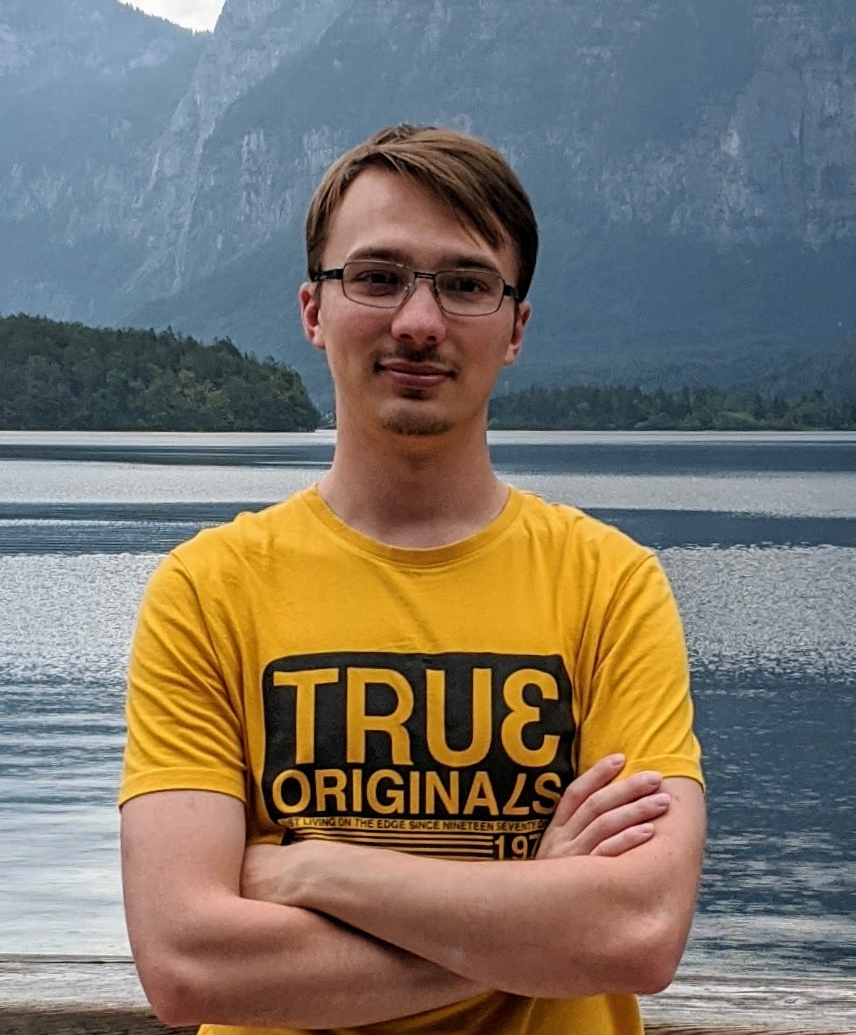
\includegraphics[width=\textwidth]{profile}
    \end{figure}
    
    \begin{center}
        Arcadii Rubailo
    
        Age: 25 August 20, 1995
    \end{center}
    
    \begin{tabular}{ c l }
        \icon{icon_email}           &   rubailo.arcadii@gmail.com       \rowend
        \icon{icon_phone}           &   +420 775 087 503                \rowend
        \icon{icon_home}            &   Videnska 22d, Brno              \\
                                    &   Czech Republic                  \rowend
        \icon{icon_flag}            &   Moldova                         \rowend                        
        \icon[15pt]{icon_linkedin}  &   /arcadii-rubailo                \rowend
        \icon[18pt]{icon_github}    &   /elderanakain                   \rowend
        \icon{icon_list}            &   Programming languages:          \\
                                    &   Kotlin, Java.                   \\
                                    &   Development tools:              \\
                                    &   Android Studio, IntelliJ IDEA,  \\
                                    &   Zeplin, Jira, Figma.            \\
        \icon{icon_language}        &   \begin{tabular}{ l l }          \\
                                            Russian     &   Native      \\
                                            English     &   C1          \\
                                            Romanian    &   B1          \\
                                            Czech       &   A1          \\
                                        \end{tabular}                   \rowend
    \end{tabular}
\end{minipage}
\hspace{15pt}
\begin{minipage}[t]{0.6\textwidth}
    \sectionTitle{Education}{icon_school}
    
    \subsectionTitle{Masaryk University – MSc} \hfill 2017 – 2019
    
    Faculty of Informatics \newline
    Service Science, Management and Engineering programme
    
    \subsectionTitle{State University of Moldova – BSc} \hfill 2014 – 2017
    
    Mathematics and Computer Science \newline
    Computer science programme \newline
    
    \sectionTitle{Experience}{icon_work}
    
    \subsectionTitle{Kiwi.com} \hfill 07.2018 – Present
    
    Kiwi.com Android app, booking main developer. \newline
    Tech stack: Kotlin/Java, MVVM, Realm, ARCore (OpenGL), \newline
    Dagger2/Koin, Databinding\&LiveData, Moshi/Gson, \newline
    RxJava2/Flow, Jetpack Libraries, Retrofit2+OkHttp3.
    
    \subsectionTitle{Ellation} \hfill 01.2017 – 08.2017
    
    VRV and Crunchyroll Android apps development.
    Tech stack: Java/Kotlin, Retrofit2+OkHttp3, Chromecast, MVP, Fabric, Exoplayer, Firebase, Branch.io, Outbound.io, JUnit4, Mockito1.
   
    \subsectionTitle{Yopeso} \hfill 08.2016 – 01.2017
    
    limango Android app development. \newline
    Tech stack: Java, Retrofit+OkHttp3, Firebase, RxJava, MVP, \newline
    JUnit4+Mockito2, Dagger2, SQLite.
    
    \subsectionTitle{Travod International} \hfill 10.2015 – 08.2016
    
    Technical support, DTP and project management. \newline
    Tech stack: Photoshop, InDesign, SDL Trados.
    
    \subsectionTitle{Aursoft} \hfill 02.2015 – 12.2015
    
    MyBebe Android app development. \newline
    Tech stack: Java, Support Library, Volley, Picasso, SQLite.

    \subsectionTitle{Hobbies and interests}
    
    Reading: science fiction, IT blogs, self-development. \newline
    Master of sports in archery.
\end{minipage}
\end{document}
